\chapter{Grundlegende Begriffe}
\label{ch:basics}
In folgendem Kapitel werden die Grundlagen erläutert, welche für spätere Kapitel benötigt werden. 
Es wird kurz auf die Historie von Turing Tests eingegangen, um die grundlegende Funktionsweise von CAPTCHAs zu erklären.
Anschließend werden die verschiedenen CAPTCHA-Methoden und Alternativen grundlegend erläutert. 

Hierbei werden bereits einige Techniken aussortiert, da diese aus verschiedenen Gründen nicht relevant für die spätere Betrachtung sind.
Zuletzt wird ein grundlegendes Verständnis für UX geschaffen.

\section{Turing Tests}
\label{ch:basics:turing}
Alan M. Turing $($1912-1954$)$ ist einer der Mitbegründer der heutigen Informatik 
und legte mit seiner Forschung einen der Grundsteine für die Entwicklung von künstlicher Intelligenz. 
In seinem Paper ''On computable numbers, with an application to the Entscheidungsproblem'' \cite{turing} 
beschreibt er den Umgang mit ''computable numbers'' und wie diese durch eine - später als Turing Machine bezeichnete - Maschine berechnet werden könnte.
Diese Turing Machine ''[\dots] ist damit ein Model physischer digitaler Computer, die zu jener Zeit jedoch noch nicht existieren. [\dots]'' \cite[p.4]{pallay2020turing}
Hierbei kam er zur Erkenntnis, dass sich nicht alle mathematischen Probleme durch eine fixe Vorgehensweise, also einen Algorithmus, lösen lassen. 
Erst später wurde festgestellt, dass Turing Maschinen und Computer jeweils vom anderen simuliert werden können. \cite[p.647]{geniusofturing} \cite[p.4]{pallay2020turing} %TODO: Formulierung

Turing beschäftigte sich bis zu seinem frühen Tod weiterhin mit maschineller Intelligenz 
und ''[\dots] beschreibt [\dots] das, was man heute als [\dots] künstliche Intelligenz bezeichnet.'' \cite[p.10]{pallay2020turing}

Durch seine Überzeugung, dass eines Tages maschinelle Intelligenzen entwickelt werden (können), 
entwickelte Turing in seinem Paper ''Computing Machinery and Intelligence'' \cite[p.23ff]{turing2009computing} 
eine Methode des Testens der Intelligenz einer Maschine. 
Um die Notwendigkeit von genauen Definitionen zu vermeiden, nutzt er deshalb eine Abwandlung eines Verfahren - das ``imitation game''. 
''Hierbei kommuniziert ein Juror maschinen-schriftlich mit einem Menschen und einer Maschine.'' \cite[p.12]{pallay2020turing}
Sollte der Juror nicht feststellen können, welcher Gesprächspartner der Mensch ist, gilt der Test als bestanden. \cite[p.11ff]{pallay2020turing}

Die Idee dieses Verfahrens wird heute in sogenannten Turing Tests verwendet.
Bei dem Juror kann es sich auch um einen anderen Computer handeln.

\pagebreak

\section{CAPTCHA}
\label{ch:basics:captcha}
Bei der Abkürzung CAPTCHA handelt es sich um ''completely automated public turing tests to tell computers and humans apart''. 
Sie werden genutzt, um Webseiten vor unerwünschten, eventuell böswilligen Aktionen durch Bots zu schützen. 
Bots sind Computerprogramme, welche automatisiert Algorithmen abarbeiten und dabei unter anderem Eingaben tätigen.
Solche Aktionen können beispielsweise Spam- oder 
DDoS-Attacken\footnote[1]{Distributed Denial of Service (DDoS): Ausfälle von Systemen durch eine sehr hohe Menge von Anfragen, 
welche aufgrund ihrer Fülle nicht zeitnah abgearbeitet werden können.} sein.
Dies wird durch die im vorherigen Kapitel bereits erläuterten Turing Tests erreicht. 
Hier ist das Ziel, durch für Computer schwer, für Menschen jedoch leicht zu verarbeitende Medien, das Tracken von Mausbewegungen
oder auch das Prüfen der Browseraktivität zu testen, ob es sich wirklich um eine menschliche Nutzer*in handelt.
Genutzt werden diese CAPTCHAs beispielsweise in Kommentarbereichen, bei der Registrierung auf Webseiten,
bei Umfragen oder vor der Einsicht kritischer Daten, wie öffentlich geposteten E-Mail-Adressen. (Vgl. \cite{moradi})

Als Synonym zu CAPTCHA kann HIP verwendet werden - ''Human Interactive Proofs''. 

\subsection{Arten von CAPTCHA}
\label{ch:basics:captcha:arten}
Nachfolgend werden verschiedene Arten von CAPTCHAs grundlegend erläutert.
Dabei werden verschiedene Methoden und Techniken kurz erklärt. 
Eine genaue Vorstellung spezifischer Produkte des freien Markts findet nicht statt.
Eventuelle Sicherheitslücken in spezifischen Systemen werden in \autoref{ch:bewertung} erläutert.

\subsubsection*{Textbasierte CAPTCHA}
Textbasierte CAPTCHA waren 2008 die am häufigsten verwendete Art von CAPTCHA.
Sie zeichnen sich durch eine Verzerrung eines Wortes oder mehreren Wörtern aus, sodass diese für Bilderkennungstools nicht erkennbar sind.
Eine weitere Variante textbasierter CAPTCHA ist die einer einfachen Rechenaufgabe. 
Auch hier soll erreicht werden, dass ein Bot die angegebenen Zahlen nicht korrekt erkennen kann und die Gleichung somit nicht lösen kann. \cite[p.1]{usabilityofcaptchas} \cite[p.75]{surveyofresearch} \cite{shinde2018DIFFERENTTO} %TODO SEITEN!!!!!!!!!

Bei der Darstellung dieser Zeichen und Symbole können verschiedene Ansätze verfolgt werden.
\citeauthor{surveyofresearch} beschreiben hierbei ``anti-segmentation techniques'' und ``anti-recognition techniques''. \cite[p.76]{surveyofresearch}

\begin{figure}[h!]
    \centering
    \subfloat[\centering]{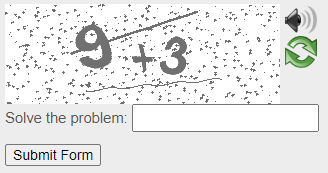
\includegraphics[width=6cm]{gfx/mygraphics/maths.png}}
    \qquad
    \subfloat[\centering]{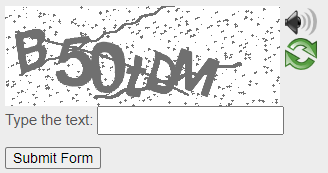
\includegraphics[width=6cm]{gfx/mygraphics/textbased.png}}
    \caption{Textbasierte CAPTCHAs aus der Securimage phpCaptcha Demo}   
    \label{fig:textbased}
\end{figure}

Anti-Segmentation Techniques zielen darauf ab, das Separieren der einzelnen Buchstaben durch Algorithmen zu erschweren. 
Um dies zu erreichen, gibt es verschiedene Herangehensweisen.
Eine von ihnen besteht daraus, dass nur die Konturen der verschiedenen Zeichen angezeigt werden, sodass diese nur von Menschen erkannt werden können,
Bots hingegen wenig Chancen haben, diese korrekt zu unterscheiden. Diese Art von CAPTCHA nennen \citeauthor{surveyofresearch} ``Hollow CAPTCHAs''. %Formulierung
Eine weitere Methode ist, Zeichen nah beieinander oder sogar überlappend darzustellen, 
was von \citeauthor{surveyofresearch} als ``crowing characters together $($CCT$)$ and overlapping'' bezeichnet wird.
Auch unruhige Hintergründe können Segmentierung behindern.
Ebenfalls beschrieben wird die Kombination von mehreren der beschriebenen CAPTCHAs zu einer ``two-layer'' Struktur,
wobei die Tatsache, dass es sich um mehrere Zeilen Text handelt, nicht erkannt werden kann. \cite[p.76]{surveyofresearch} \cite[p.132f]{Beheshti}

Anti-Recognition Techniques sind zum Beispiel verschiedene Schriftarten, die Rotation von Zeichen und ``Waving'', 
welche es erschweren, Zeichen als solche zu erkennen. 
Außerdem können in einigen Fällen auch sehr große Zeichensätze, beispielsweise Mandarin oder Japanisch, genutzt werden, 
wodurch das Finden von eindeutigen Lösungen erschwert werden kann.
Diese Techniken werden oftmals miteinander kombiniert.
\cite[p.77]{surveyofresearch}

Eine Kombination von Anti-Segmentation und Anti-Recognition Techniken ist in \autoref{fig:textbased} zu sehen.

\begin{figure}[h!]
    \centering
    \subfloat[\centering]{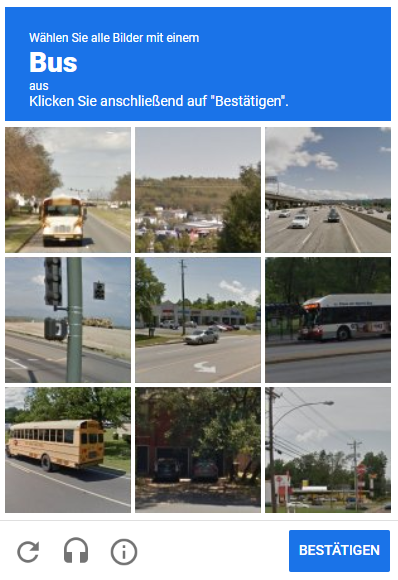
\includegraphics[width=6cm]{gfx/mygraphics/selectionbasedrecaptcha.png}}
    \qquad
    \subfloat[\centering]{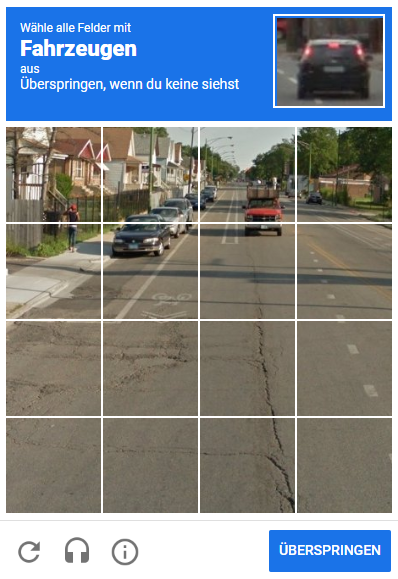
\includegraphics[width=6cm]{gfx/mygraphics/selectionbasedrecaptcha2.png}}
    \caption{Bildbasierte CAPTCHAs nach unzureichendem Score bei der Bewertung durch reCAPTCHA v2}   
    \label{fig:selectionbased}
\end{figure}

\subsubsection*{Bildbasierte CAPTCHA}
Es gibt verschiedene Arten von bildbasierten CAPTCHAs. 
Die wohl bekannteste ist ein in Quadrate aufgeteiltes Bild, wobei man jene Quadrate auswählen soll, welche einen bestimmten Gegenstand enthalten.
Eine Variation dieses CAPTCHAs besteht aus einer Zahl verschiedener Bilder, von denen eine Teilmenge ebenfalls ein gesuchtes Objekt beinhalten 
und sich semantisch ähneln. 
\autoref{fig:selectionbased} stellt diese Variationen dar.
In Abbildung \ref{fig:fortnite} sollen Hunde mit geschlossenen Augen ausgewählt werden,
was die Notwendigkeit der Zunahme der Komplexität dieser CAPTCHAs gut widerspiegelt. 
Außerdem kann auch auf das Erkennen von Gesichtern durch Menschen gesetzt werden.
Nähere Informationen zu genauen Techniken können in \cite[p.77ff]{surveyofresearch} nachgelesen werden.
Die beschriebenen ``selection-based CAPTCHA'' bezeichnen \citeauthor{surveyofresearch} als einfachste Form bildbasierter CAPTCHA. \cite[p.77]{surveyofresearch}

In Abbildung \ref{fig:genshin} sind zwei weitere Arten bildbasierter CAPTCHA dargestellt.
Links ist ein ``drag-based CAPTCHA'' zu sehen.
Hierbei werden Mausbewegungen, die Geschwindigkeit dieser Bewegungen
und die allgemeine Reaktionszeit überprüft.
Dies geschieht, wie in Abbildung \ref{fig:genshin} (a) zu sehen,
beispielsweise über das Verschieben eines Puzzleteils an die richtige Stelle.
Andere Variationen dieser CAPTCHA-Art verlangen, dass ein Bild mithilfe eines Schiebereglers in die richtige Position gebracht,
oder eine Kontur oder Bewegung mit der Maus nachverfolgt werden soll.
Auch hier kann in \cite[p.77]{surveyofresearch} genauer nachgelesen werden.

\begin{figure}[h!]
    \centering
    \subfloat[\centering]{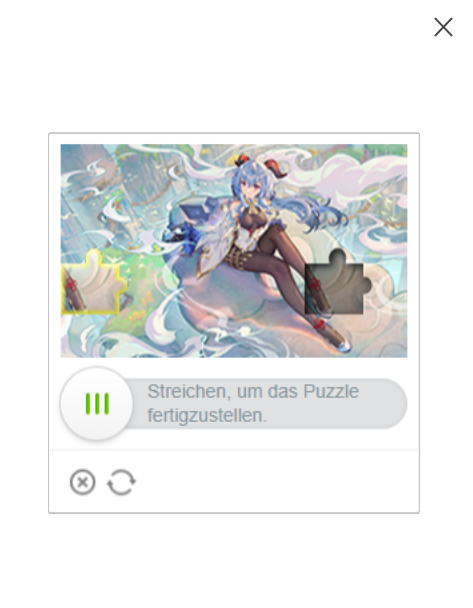
\includegraphics[width=6cm]{gfx/mygraphics/genshincaptcha.png}}
    \qquad
    \subfloat[\centering]{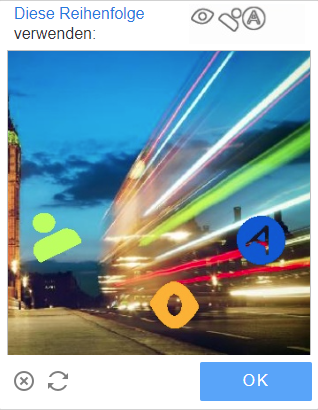
\includegraphics[width=6cm]{gfx/mygraphics/hoyoversecaptcha.png}}
    \caption{Bildbasierte CAPTCHA von GeeTest bei Login in Genshin Impact $($a$)$ und dem Forum Hoyolab $($b$)$}   
    \label{fig:genshin}
\end{figure}

``Click-based CAPTCHA'' zeichnen sich dadurch aus, dass bestimmte Symbole oder Zeichen auf einem komplexen Hinter\-grund, 
teilweise auch in einer bestimmten Reihenfolge, angeklickt werden sollen.
Hierbei wird auf ``anti-detection'' und ``anti-recognition'' gesetzt. \cite[p.77]{surveyofresearch}

Ein Beispiel hierfür ist \ref{fig:genshin} (b).
Eine weitere Form der click-basierten CAPTCHAs sieht vor, dass Objekte ausgewählt werden sollen,
die beispielsweise die gleiche Textur besitzen oder räumlich nah an einem bestimmten anderen Objekt dargestellt sind. 
Diese sind zum Beispiel VTT\footnote[2]{VTT = Visual Turing Test} CAPTCHA. (Vgl. \cite[p.78]{surveyofresearch})

Ein Beispiel hierfür ist in \autoref{fig:geetest} zu sehen.
Hier wird über die Größe, Farbe und Position angegeben, welches Objekt angeklickt werden muss, um den CAPTCHA zu lösen.
Die Formulierung ``in front of'' ist hierbei auch auf Objekte bezogen, die nicht genau, sondern auch versetzt, vor dem gelben Zylinder stehen.
Zum Lösen des CAPTCHAs muss deshalb auf die grüne Kugel geklickt werden.

\begin{figure}[h!]
        \centering
        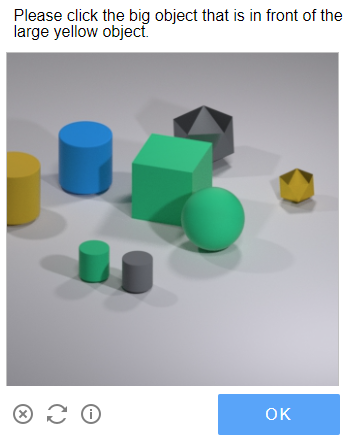
\includegraphics[width=6cm]{gfx/mygraphics/raeumlich.png} 
    \caption{Bildbasierter CAPTCHA aus der GeeTest Demo}
    \label{fig:geetest}
\end{figure}

\subsubsection*{Gamification}
Bei Gamification CAPTCHAs liegt der Fokus darauf, eventuell langwieriges Ausfüllen von CAPTCHAs so zu gestalten, dass Nutzer*innen dabei Spaß haben,
und es nicht als lästige Aufgabe ansehen.
\citeauthor{gamified} schreiben in ihrem Paper \citetitle{gamified} darüber, wie spielerisch lösbare CAPTCHAs die Nutzererfahrung verbessern können.
Hierbei werden Ideen wie das Ordnen von Cartoon-Panelen näher erläutert.
\pagebreak

Nicht nur lesen Nutzer*innen den Cartoon, sie wollen bei Fehlschlägen durch den Quizcharakter des CAPTCHAs die richtige Lösung in einem weiteren Versuch finden,
ohne über die Notwendigkeit der Wiederholung zur Verifizierung nachzudenken. \cite[p.41ff]{gamified}


\subsubsection*{Videobasierte CAPTCHA}
Eine weitere Form visueller CAPTCHAs sind videobasierte CAPTCHA. 
Nutzer*innen müssen beispielsweise verschiedene Bewegungen erkennen, die im Video ausgeführt werden,
oder auch angezeigte Werbung.
Dabei werden verschiedene Antwortmöglichkeiten vorgegeben, welche durch Raten auch durch Bots erfolgreich absolviert werden können.
Um dies zu umgehen gibt es Alternativen, die über das Beschreiben des gesehenen Videos funktionieren. \cite[p.79]{surveyofresearch} 

\subsubsection*{Audiobasierte CAPTCHA}
Als Alternative von visuellen CAPTCHAs können audiobasierte CAPTCHA genutzt werden.
Diese bieten sich vor allem für sehbehinderte Nutzer*innen an, welche bild- oder textbasierte CAPTCHA nur schwer oder gar nicht sehen und erkennen können.

Oft wird hier Text-To-Speech verwendet, wobei die gehörten Wörter durch die Nutzer*innen wiederholt werden sollen.
Eine weitere Möglichkeit ist das Abspielen bestimmter Töne, wie die einer Glocke oder eines Klaviers. 
Dies kann auch in Kombination mit verschiedenen Hintergrundgeräuschen angewandt werden, was das Erkennen eines bestimmten Tons für Roboter zusätzlich erschwert.
Außerdem gibt es Methoden, bei denen eine bestimmte Frage beantwortet werden muss, für die gesunder Menschenverstand notwendig ist. 
Beispielsweise kann nach einer Aussage wie ``Sally hat einen Nagel in den Boden gehämmert.'' gefragt werden, ob dieser Nagel vertikal oder horizontal war. \cite[p.3]{commonsense}

Neben Techniken, die hauptsächlich auf das Hören ausgelegt sind, kann der Fokus auch auf das Einsprechen von Phrasen durch die Nutzer*innen gelegt werden.
Es soll so erkannt werden, ob es sich um eine menschliche Stimme handelt.
\cite[p.78]{surveyofresearch}

\begin{figure}[h!]
    \centering
    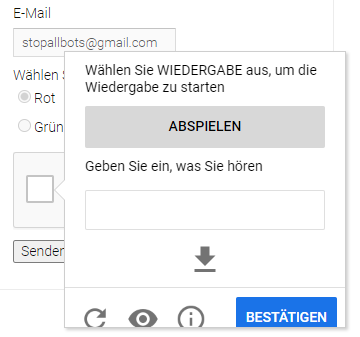
\includegraphics[width=6cm]{gfx/mygraphics/audio.png}
     \caption{Audiobasierte Alternative zu bildbasiertem CAPTCHA von reCAPTCHA v2}
      \label{fig:audio}
\end{figure}

\pagebreak

\subsection{Alternativen zu klassischen CAPTCHA}
\label{ch:basics:captcha:alternativen}
Neben klassischen Turing Tests gibt es weitere Möglichkeiten, Roboter und Menschen zu unterscheiden.
Aus diesem Grund werden nachfolgend Alternativen zu klassischen CAPTCHAs vorgestellt.

\subsubsection*{CAPTCHA mit minimalem User-Input}
Eine aktuell viel genutzte Form der Spam-Prävention ist reCAPTCHA v3 von Google. 
Hier werden keine klassischen Turing Tests durchgeführt. 
Vielmehr wird anhand verschiedener Faktoren bewertet, ob es sich um einen Bot oder einen Menschen handelt.
Die Betrachtung von Cookies oder der Häufigkeit von Anfragen durch die gegebene IP-Adresse werden hierbei unter anderem betrachtet.
In der Dokumentation wird angegeben, dass ein Score von 0.0 bis 1.0 vergeben werden kann. 
Hier gilt: Je niedriger der Score, desto wahrscheinlicher handelt es sich um einen Bot statt einer echten Nutzer*in. (Vgl. \cite{recaptchadoc})
Laut Google selbst soll reCAPTCHA v3 eine sehr gute Nutzererfahrung bieten, da es kaum bis gar keine Zuarbeit durch den Nutzer verlangt. \cite{googleblog:recaptcha}

ReCAPTCHA kann durch das Fehlen eines klassischen Turing Tests auch als eine CAPTCHA-Alternative interpretiert werden.

Ähnliche ``Invisible CAPTCHA''-Techniken werden auch von GeeTest \linebreak(\cite{geetest}) und hCaptcha (\cite{hcaptcha}) angeboten.

\begin{figure}[h!]
    \centering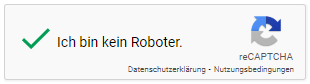
\includegraphics[width=6cm]{gfx/mygraphics/recaptcha.png}
     \caption{CAPTCHA mit wenig benötigtem User-Input - reCAPTCHA v2}
      \label{fig:recaptcha}
\end{figure}

\pagebreak

Neben CAPTCHAs ohne jegliche Interaktion gibt es auch solche, 
die über das einfache Abhaken einer Checkbox verifizieren, ob es sich um einen Roboter handelt.
Eine andere Variation verlangt von den Nutzer*innen, dass ein Button angeklickt und gehalten werden soll. 

\subsubsection*{Honeypots}
Eine weitere Alternative zu klassischen CAPTCHA sind sogenannte Honeypots. 
Geprägt wurde der Begriff erstmals im Kalten Krieg, wo diese als Spionagetechnik eingesetzt wurde. \cite[p.2]{joshi:2011} 

Auch heute werden Honeypots eingesetzt, und zwar in der IT-Sicherheit. 
Oft werden sie mit Fallen assoziiert, welche Hacker anlocken sollen. 
Dadurch können Angriffsarten analysiert werden und echte Systeme werden nicht angegriffen.

Doch auch im Kontext der Unterscheidung von Menschen und Maschine gibt es Honeypots. 
So kann man HTML-Inputfelder durch CSS oder JavaScript verstecken, sodass diese nur durch Bots, welche den Quellcode der Seite scannen, ausgefüllt werden 
und nicht durch Menschen, da diese das Textfeld nicht sehen. 
Bei der Prüfung der Inputs kann nun überprüft werden, ob ein Bot in die Falle getappt ist. 
Nachzulesen sind solche Verfahren in verschiedenen Blogposts, wie \cite{perry:2019}.

\subsubsection*{Anti-Spam-Plugins}
Anti-Spam-Plugins können anstelle von CAPTCHAs genutzt werden, wenn man beispielsweise Kommentar\-bereiche moderieren möchte.
Das WordPress-Plugin ``Antispam-Bee'' arbeitet auf Basis verschiedener Anhaltspunkte, 
welche Auskunft darüber geben können, ob es sich bei Nutzer*innen wirklich um einen Menschen handelt.
Es kann beispielsweise überprüft werden, ob Kommentator*innen Gravatar
\footnote[3]{Gravatar steht für "Globally Recognized Avatar". 
Es kann ein Profilbild hochgeladen werden, welches mit einer oder mehreren E-Mail-Adressen verknüpft ist 
und neben Kommentaren angezeigt wird, wenn dort die entsprechende E-Mail-Adresse angegeben wurde. (Vgl. \cite{doku:antispambee})} nutzen.
Außerdem können IP-Adressen betrachtet werden und diese kann neben anderen Daten der Kommentator*innen gegebenenfalls in ``Spamdatenbanken'' gefunden werden.
Auch das Blockieren von Kommentaren aus bestimmten Ländern oder das Akzeptieren von Kommentaren in ausschließlich einer Sprache ist möglich.
Dieses Plugin und die beschriebenen Maßnahmen zur Spam-Präventionen sind nur eine von vielen Optionen, die hier zur Verfügung stehen.
\cite{blog:antispambee}
\cite{doku:antispambee}

\subsubsection*{Multi-Faktor-Authentifikation}
Die Authentifikation von Nutzer*innen über mehrere Schritte kann genutzt werden, um die unbefugte Nutzung von Accounts und Ähnlichem zu verhindern.
Dadurch kann beispielsweise verhindert werden, dass gestohlene Accountdaten für Spamangriffe genutzt werden können.

Dieser zweite Schritt, der vor dem Login durchgeführt werden muss, ist beispielweise das Anklicken eines Links oder das Eingeben eines Codes,
welcher über eine App oder SMS zugeschickt wurde.
Jedoch ersetzt dies nicht das Ausfüllen von CAPTCHAs.
Auch ein Algorithmus kann diese Aktionen mit Leichtigkeit ausführen. 
Die Nutzung von Multi-Faktor-Authentifikation ist zwar nicht schlecht,
bietet aber keine adäquate Alternative zu der Nutzung von CAPTCHAs. 
Aus diesem Grund wird die Multi-Faktor-Authentifi\-kation in Folgendem nicht weiter betrachtet.

\subsubsection*{Biometrie}
Eine relativ neue Art der Überprüfung von Nutzer*innen ist die Verifizierung durch Biometrie.
Hierbei wird über das Scannen des Gesichts oder die Erkennung einer Stimme entschieden, ob es sich wirklich um einen (bestimmten) Menschen handelt.
In \cite{rtcaptcha} wird diese Technik näher erläutert. 

Biometrische Verfahren werden hauptsächlich als eine Variation der Multi-Faktor-Authentifikation genutzt,
weshalb sie folgend nicht berücksichtigt werden. 

\section{User Experience}

User Experience (UX) beschreibt die Erfahrungen eines Users bei der Nutzung eines Systems. 
Das Ziel ist, diese Nutzererfahrung möglichst positiv zu halten. 
Im Kontext dieser Ausarbeitung wird die Definition des  ``international standard on ergonomics of human-system interaction'' $($ISO 9241-210$)$
aus dem Jahre 2010 verwendet. 
Diese definitiert UX als die Wahrnehmungen und Resonanzen einer Person, 
welche aus der $($voraussichtlichen$)$ Nutzung eines Produkts, Systems oder Services entstehen. \cite[p.1629]{berni_borgianni_2021}

Die Nutzererfahrung bei der Wahl und Nutzung von CAPTCHA ist neben der Sicherheit ein essentieller Bestandteil.
Bei der Entwicklung einer Bewertungsmatrix soll deshalb hier der Hauptfokus liegen.
Denn wenn ein CAPTCHA schwierig zu lösen ist, oder von bestimmten Personengruppen gar nicht bearbeitet werden kann, so stört dies nicht nur den Nutzungsfluss,
sondern führt gegebenenfalls auch dazu, dass Nutzer*innen die Seite verlassen, ohne ihre gewünschte Aktion zu vollenden. 
